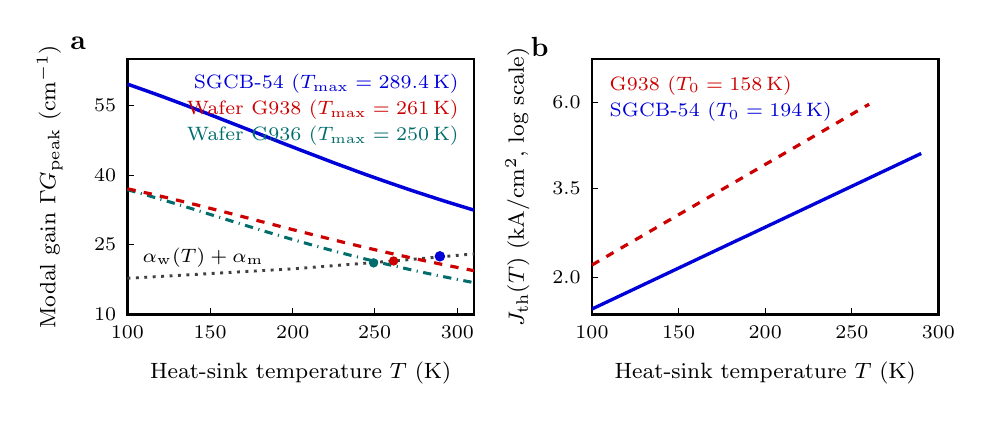
\begin{tikzpicture}[x=1cm,y=1cm,font=\footnotesize]
  % Panel a: Modal gain G_M(T) vs Cu-Cu waveguide loss
  \node[anchor=north west,font=\bfseries\normalsize] at (0.10,4.35) {a};
  \draw[thick] (0.95,0.70) rectangle (5.35,3.95);
  \foreach \v/\y in {10/0.70, 25/1.59, 40/2.47, 55/3.36} {
    \draw (0.95,\y) -- (1.03,\y);
    \node[left,font=\scriptsize] at (0.93,\y) {\v};
  }
  \foreach \xval/\xpos in {100/0.95, 150/2.00, 200/3.05, 250/4.09, 300/5.14} {
    \draw (\xpos,0.70) -- (\xpos,0.78);
    \node[below,font=\scriptsize] at (\xpos,0.68) {\xval};
  }
  \node[below,font=\footnotesize] at (3.15,0.22) {Heat-sink temperature $T$ (K)};
  \node[rotate=90,above,font=\footnotesize] at (0.25,2.32) {Modal gain $\Gamma G_{\mathrm{peak}}$ ($\mathrm{cm}^{-1}$)};

  \draw[black!75,dotted,line width=1.05pt] (0.95,1.16) -- (3.05,1.28) -- (4.33,1.38) -- (5.35,1.47);
  \node[anchor=south west,font=\scriptsize] at (1.02,1.18) {$\alpha_{\mathrm{w}}(T)+\alpha_{\mathrm{m}}$};

  \draw[teal!85!black,dashdotted,line width=1.1pt] (0.950,2.285) -- (1.055,2.256) -- (1.160,2.226) -- (1.264,2.196) -- (1.369,2.165) -- (1.474,2.134) -- (1.579,2.102) -- (1.683,2.070) -- (1.788,2.038) -- (1.893,2.005) -- (1.998,1.972) -- (2.102,1.940) -- (2.207,1.907) -- (2.312,1.874) -- (2.417,1.842) -- (2.521,1.810) -- (2.626,1.778) -- (2.731,1.746) -- (2.836,1.715) -- (2.940,1.684) -- (3.045,1.654) -- (3.150,1.624) -- (3.255,1.594) -- (3.360,1.565) -- (3.464,1.536) -- (3.569,1.508) -- (3.674,1.481) -- (3.779,1.453) -- (3.883,1.427) -- (3.988,1.401) -- (4.093,1.375) -- (4.198,1.350) -- (4.302,1.325) -- (4.407,1.301) -- (4.512,1.277) -- (4.617,1.254) -- (4.721,1.231) -- (4.826,1.209) -- (4.931,1.187) -- (5.036,1.166) -- (5.140,1.145) -- (5.245,1.125) -- (5.350,1.105);
  \draw[red!80!black,dashed,line width=1.15pt] (0.950,2.297) -- (1.055,2.274) -- (1.160,2.251) -- (1.264,2.228) -- (1.369,2.203) -- (1.474,2.179) -- (1.579,2.153) -- (1.683,2.128) -- (1.788,2.102) -- (1.893,2.076) -- (1.998,2.049) -- (2.102,2.023) -- (2.207,1.996) -- (2.312,1.969) -- (2.417,1.942) -- (2.521,1.915) -- (2.626,1.887) -- (2.731,1.860) -- (2.836,1.833) -- (2.940,1.806) -- (3.045,1.779) -- (3.150,1.753) -- (3.255,1.726) -- (3.360,1.700) -- (3.464,1.674) -- (3.569,1.648) -- (3.674,1.622) -- (3.779,1.597) -- (3.883,1.572) -- (3.988,1.548) -- (4.093,1.523) -- (4.198,1.499) -- (4.302,1.475) -- (4.407,1.452) -- (4.512,1.429) -- (4.617,1.406) -- (4.721,1.384) -- (4.826,1.362) -- (4.931,1.340) -- (5.036,1.319) -- (5.140,1.298) -- (5.245,1.278) -- (5.350,1.257);
  \draw[blue!85!black,line width=1.25pt] (0.950,3.626) -- (1.055,3.589) -- (1.160,3.552) -- (1.264,3.515) -- (1.369,3.477) -- (1.474,3.438) -- (1.579,3.399) -- (1.683,3.360) -- (1.788,3.320) -- (1.893,3.280) -- (1.998,3.239) -- (2.102,3.198) -- (2.207,3.157) -- (2.312,3.116) -- (2.417,3.075) -- (2.521,3.034) -- (2.626,2.993) -- (2.731,2.951) -- (2.836,2.910) -- (2.940,2.869) -- (3.045,2.829) -- (3.150,2.788) -- (3.255,2.748) -- (3.360,2.708) -- (3.464,2.668) -- (3.569,2.628) -- (3.674,2.589) -- (3.779,2.551) -- (3.883,2.512) -- (3.988,2.474) -- (4.093,2.437) -- (4.198,2.400) -- (4.302,2.364) -- (4.407,2.328) -- (4.512,2.292) -- (4.617,2.257) -- (4.721,2.223) -- (4.826,2.189) -- (4.931,2.155) -- (5.036,2.122) -- (5.140,2.090) -- (5.245,2.058) -- (5.350,2.026);

  \fill[teal!85!black] (4.076,1.356) circle (1.7pt);
  \fill[red!80!black] (4.330,1.380) circle (1.7pt);
  \fill[blue!85!black] (4.918,1.439) circle (1.9pt);

  \node[anchor=north east,font=\scriptsize,blue!85!black] at (5.28,3.88) {SGCB-54 ($T_{\max}=289.4\,\mathrm{K}$)};
  \node[anchor=north east,font=\scriptsize,red!80!black] at (5.28,3.55) {Wafer G938 ($T_{\max}=261\,\mathrm{K}$)};
  \node[anchor=north east,font=\scriptsize,teal!85!black] at (5.28,3.22) {Wafer G936 ($T_{\max}=250\,\mathrm{K}$)};

  % Panel b: Threshold current density & T_0 extraction
  \node[anchor=north west,font=\bfseries\normalsize] at (5.95,4.35) {b};
  \draw[thick] (6.85,0.70) rectangle (11.25,3.95);
  \foreach \lbl/\y in {2.0/1.17, 3.5/2.30, 6.0/3.39} {
    \draw (6.85,\y) -- (6.93,\y);
    \node[left,font=\scriptsize] at (6.83,\y) {\lbl};
  }
  \foreach \xval/\xpos in {100/6.85, 150/7.95, 200/9.05, 250/10.15, 300/11.25} {
    \draw (\xpos,0.70) -- (\xpos,0.78);
    \node[below,font=\scriptsize] at (\xpos,0.68) {\xval};
  }
  \node[below,font=\footnotesize] at (9.05,0.22) {Heat-sink temperature $T$ (K)};
  \node[rotate=90,above,font=\footnotesize] at (6.18,2.32) {$J_{\mathrm{th}}(T)$ ($\mathrm{kA/cm^2}$, log scale)};

  \draw[red!80!black,dashed,line width=1.15pt] (6.850,1.329) -- (6.960,1.393) -- (7.070,1.457) -- (7.180,1.521) -- (7.290,1.585) -- (7.400,1.648) -- (7.510,1.712) -- (7.620,1.776) -- (7.730,1.840) -- (7.840,1.904) -- (7.950,1.968) -- (8.060,2.031) -- (8.170,2.095) -- (8.280,2.159) -- (8.390,2.223) -- (8.500,2.287) -- (8.610,2.350) -- (8.720,2.414) -- (8.830,2.478) -- (8.940,2.542) -- (9.050,2.606) -- (9.160,2.669) -- (9.270,2.733) -- (9.380,2.797) -- (9.490,2.861) -- (9.600,2.925) -- (9.710,2.988) -- (9.820,3.052) -- (9.930,3.116) -- (10.040,3.180) -- (10.150,3.244) -- (10.260,3.308) -- (10.370,3.371);
  \draw[blue!85!black,line width=1.2pt] (6.850,0.770) -- (6.960,0.822) -- (7.070,0.874) -- (7.180,0.926) -- (7.290,0.978) -- (7.400,1.030) -- (7.510,1.082) -- (7.620,1.134) -- (7.730,1.186) -- (7.840,1.238) -- (7.950,1.290) -- (8.060,1.342) -- (8.170,1.394) -- (8.280,1.446) -- (8.390,1.498) -- (8.500,1.550) -- (8.610,1.602) -- (8.720,1.654) -- (8.830,1.705) -- (8.940,1.757) -- (9.050,1.809) -- (9.160,1.861) -- (9.270,1.913) -- (9.380,1.965) -- (9.490,2.017) -- (9.600,2.069) -- (9.710,2.121) -- (9.820,2.173) -- (9.930,2.225) -- (10.040,2.277) -- (10.150,2.329) -- (10.260,2.381) -- (10.370,2.433) -- (10.480,2.485) -- (10.590,2.537) -- (10.700,2.589) -- (10.810,2.641) -- (10.920,2.693) -- (11.030,2.745);

  \node[anchor=north west,font=\scriptsize,red!80!black] at (6.95,3.86) {G938 ($T_0 = 158\,\mathrm{K}$)};
  \node[anchor=north west,font=\scriptsize,blue!85!black] at (6.95,3.52) {SGCB-54 ($T_0 = 194\,\mathrm{K}$)};
\end{tikzpicture}
